This section describes the purpose, use and intended user audience for the Groco product. Groco is a grocery shopping application that is compatible with iOS, Android, and web. The user of Groco will be able to search for the grocery items and based on the user's preference such as locations and brands, the system will suggest the best places to shop these items with the lowest prices and fastest route. The system also allow user to search for recipes, add their own recipes and meal plans into their shopping list to perform the optimization and navigation route. 

\subsection{Purpose and Use}
The purpose of this product is to help the users save money and time shopping for groceries as well as providing the convenience in planing their meals. The product provide the optimal suggestion based on the database and is not responsible for the accuracy or changes regarding prices and discounts at the actual stores.  

\subsection{Intended Audience}
The application is an web application and users can access the application from multiple devices. The product is made available publicly and free of charge. The product contain no objectionable material; therefore it is suitable for general grocery shoppers at all ages.

\begin{figure}[h!]
	\centering
   	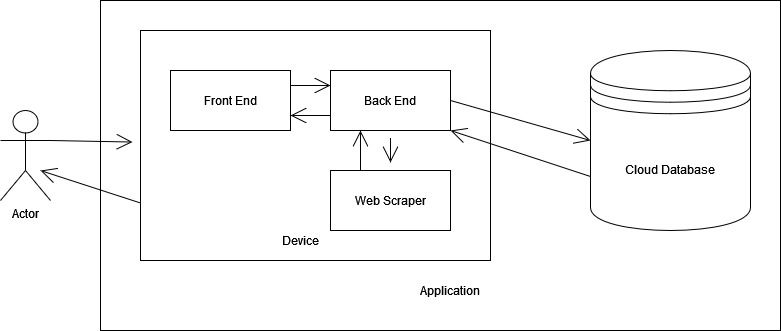
\includegraphics[width=1\textwidth]{images/system_diagram.jpg}
    \caption{High level overview of the system}
\end{figure}
